\section{Introduction and Goals}

According to the \acrfull{fao} in 2019 931 millions tonnes of food were wasted \cite{refart:FAOFW}. This has
environmental, but special social consequences. In a world were approximately 9.9\% of the \cite{refart:AAHWH}
population suffers from hunger that waste percentage sounds paradoxal.

According to \acrfull{un} 5\% of the globally food loss and waste comes from restaurants \cite{refart:UNSP}. 
The solution for this problem muss be locally applied so its effects can be seen in a global structure. To do so we
propose to develop a mobile application that connects restaurants, bakeries and or pastries to clients. 
The former would offer their remaining products, which are still consumable, prior to the closing time, to a small price 
and the latter would browser in the app to find which shops are offering products. 

 
\subsection{Design Purpose}

The main purpose of this architecture is creating exploratory prototype. We aim to test it with potential users and
regions to analyze the general acceptance and wishes of our stakeholders \cite{refbook:DSHC} and get a fast feedback. 

This prototype will also make it feasible to identify unknown needs an wishes of the potential users, so we can eventually
increase the scope of functionality. Exploring this domain will also provide us with information regarding the behavior 
of our users when it comes to buying food that would be wasted, but is still consumable.

\subsection{Primary Functionality}

From the following use cases we will be able to define the primary functionality of our application and 
furthermore identify its main quality attributes 

% Object: put figure beside the table

\begin{table}[htb]
    \begin{tabularx}{\textwidth}{lX}
    \toprule
    Use Case & Description  \\
    \midrule
    UC-1: Register as client & The user register an e-mail address.\\
    UC-2: Login & The user logins in to the system. \\
    UC-3: Place order & The user chooses a provider. \\
    UC-4: Register payment & The user register a payment method. \\
    UC-5: Register as provider & The provider register their facility and products. \\
    UC-6: Update availability & The provider upload their availability to provide a product. \\
    \bottomrule
    \end{tabularx}
\end{table}

Those use cases are also represented in the following use case diagram:

\begin{figure}[htb]
    \centering
    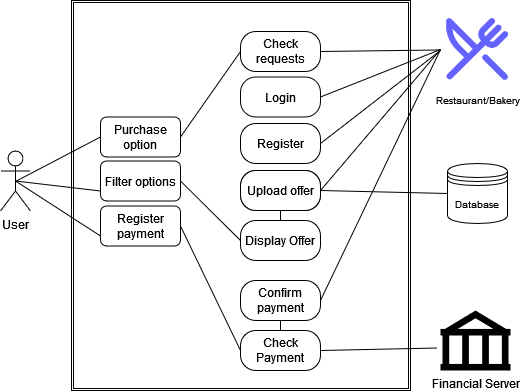
\includegraphics[width=0.50\textwidth]{/home/bruno/git/Soft.Arch/assets/preliminary_use_case.png}
    \caption{Preliminary functions}
    \label{fig:predes}
\end{figure}


\subsection{Quality Attributes}

With the given use cases we will then be able to define the major quality attributes that are involved in the 
development of this application. We want those qualities to be measurable and testable so we can verify if the 
system meets the needs our stakeholders \cite{refbook:DSHC}.

\begin{table}[H]
\begin{tabularx}{\textwidth}{lcXc}
    \toprule
    ID & Quality Attribute & Scenario & Associated Use Case  \\
    \midrule
    QA-1 & Performance & A client register their e-mail address and he can immediate browse in the app. & UC-1 \\
    QA-2 & Performance & A client opens the app and he can immediate browse in the app. & UC-2 \\
    QA-3 & Performance & A client choose a provider and place his order. After the confirmation
    of payment, a push-message is displayed in the app confirming the purchase. & UC-3 \\
    QA-4 & \textit{[to be defined]} & A client register his credit card or select another payment method and the
    confirmation as soon as he confirmed with his provider. & UC-4 \\
    QA-5 & Usability & A provider is able to register his company, specify the kind of products he offers and upload
    a logo or picture of his shop. & UC-05 \\
    QA-6 & Usability & A provider is able to update in the app if he is offering for that day any product. &  UC-6 \\
    \bottomrule
\end{tabularx}
\end{table}

The defined quality attributes are represented in the following scenarios:

\begin{table}[H]
    \begin{tabularx}{\textwidth}{|c|X|}
        \hline
        \multicolumn{2}{c}{\textbf{Performance}} \\
        \hline
        \toprule
        \multicolumn{1}{c}{Scenario} & \multicolumn{1}{c}{Value} \\
        \midrule
        Source & End user \\
        Stimulus & wishes to create an account \\
        Artifact & platform \\
        Environment & runtime \\
        Response & immediate access to the app \\
        Response Measure & time between confirmation and access \\
         & \\
        Source & End user \\
        Stimulus & wants to search fo restaurants or bakeries \\
        Artifact & platform \\
        Environment & peak period, between 6 and 7 pm on Friday \\
        Response & immediate access to the offers \\
        Response Measure & how quick does the user get an updated regarding availability of products \\
        & \\
        Source & End user \\
        Stimulus & place an order \\
        Artifact & platform \\
        Environment & peak period, between 6 and 7 pm on Friday \\
        Response & confirmation of the purchase after the payment \\
        Response Measure & time between confirmation of the payment and confirmation of the order \\
        \bottomrule
    \end{tabularx}
\end{table}

\begin{table}[H]
    \begin{tabularx}{\textwidth}{|c|X|}
        \hline
        \multicolumn{2}{c}{\textbf{Usability}} \\
        \hline
        \toprule
        \multicolumn{1}{c}{Scenario} & \multicolumn{1}{c}{Value} \\
        \midrule
        Source & Provider \\
        Stimulus & wants to offer his remaining products in the app \\
        Artifact & platform \\
        Environment & working time, during afternoon \\
        Response & offer available in the app \\
        Response Measure & How long did the registration and upload process took? Were all necessary information
        available in the app or did the provider need to search it outside the app? How long did the registration
        process took? \\
         & \\
        Source & Registered provider \\
        Stimulus & wants wants to make a last minute offer \\
        Artifact & platform \\
        Environment & peak period, between 6 and 7 pm on Friday \\
        Response & immediate availability of the offer in the app \\
        Response Measure & how long did it take for the provider to upload the offer? Was it easy to input all
        necessary information like, quantity, location and take-away time? Can he do it without any burden? \\
        \bottomrule
    \end{tabularx}
\end{table}

\subsection{Design Purpose}

\textit{to be written}

%https://medium.com/@janerikfra/architectural-drivers-in-modern-software-architecture-cb7a42527bf2 (important)
% https://www.ecs.csun.edu/~rlingard/COMP684/Example2SoftArch.htm
% https://upcommons.upc.edu/bitstream/handle/2099.1/18373/90629.pdf

% Registration Process for Clients QA1
% Registration Process for Restaurants/Backery QA2
% Login Clients QA3
% Login Restaurant/Backery QA4
% Upload offers QA6
% Purchase QA6
% Receive Confirmation QA7

% Performance
% After upload offer, how long until displyed QA8

% Usuability
% Registration for Client: using existing account or Name/email
% Registration for Restaurant/bakery: Upload name, picture, location and type of products

% Purchase client: choose available RA-options
% Payment: register card, use existing accounts (paypal/google pay)

% Upload offer RA: registered RAs activate that they are offering
% Receive order: after payment confirmed, RA recieves order


% Availability

% Modifiability
